% --------------------------------------------------------------
%                           Set Up
% --------------------------------------------------------------
 
\documentclass[12pt]{article}
 
\usepackage[margin=1in]{geometry} 
\usepackage{amsmath,amsthm,amssymb}
\usepackage{listings}
\usepackage{xcolor}
\usepackage{graphicx}
\usepackage{subcaption}
\usepackage{listings}
\usepackage{xcolor}
\usepackage{comment}
 
\definecolor{codegreen}{rgb}{0,0.6,0}
\definecolor{codegray}{rgb}{0.5,0.5,0.5}
\definecolor{codepurple}{rgb}{0.58,0,0.82}
\definecolor{backcolour}{rgb}{0.95,0.95,0.92}
 
\lstdefinestyle{mystyle}{
    backgroundcolor=\color{backcolour},   
    commentstyle=\color{codegreen},
    keywordstyle=\color{magenta},
    numberstyle=\tiny\color{codegray},
    stringstyle=\color{codepurple},
    basicstyle=\ttfamily\footnotesize,
    breakatwhitespace=false,         
    breaklines=true,                 
    captionpos=b,                    
    keepspaces=true,                 
    numbers=left,                    
    numbersep=5pt,                  
    showspaces=false,                
    showstringspaces=false,
    showtabs=false,                  
    tabsize=2
}
 
\lstset{style=mystyle}
 
\definecolor{codegreen}{rgb}{0,0.6,0}
\definecolor{codegray}{rgb}{0.5,0.5,0.5}
\definecolor{codepurple}{rgb}{0.58,0,0.82}
\definecolor{backcolour}{rgb}{0.95,0.95,0.92}
\definecolor{deepblue}{rgb}{0,0,0.5}
\definecolor{deepred}{rgb}{0.6,0,0}
\definecolor{deepgreen}{rgb}{0,0.5,0}
 
\lstdefinestyle{mystyle}{
    backgroundcolor=\color{backcolour},   
    commentstyle=\color{codegreen},
    keywordstyle=\color{deepred},
    numberstyle=\tiny\color{codegray},
    stringstyle=\color{deepblue},
    basicstyle=\ttfamily\footnotesize,
    breakatwhitespace=false,         
    breaklines=true,                 
    captionpos=b,                    
    keepspaces=true,                 
    numbers=left,                    
    numbersep=5pt,                  
    showspaces=false,                
    showstringspaces=false,
    showtabs=false,                  
    tabsize=2
}
 
\lstset{style=mystyle}
 
\newcommand{\N}{\mathbb{N}}
\newcommand{\Z}{\mathbb{Z}}
 
\newenvironment{theorem}[2][Theorem]{\begin{trivlist}
\item[\hskip \labelsep {\bfseries #1}\hskip \labelsep {\bfseries #2.}]}{\end{trivlist}}
\newenvironment{lemma}[2][Lemma]{\begin{trivlist}
\item[\hskip \labelsep {\bfseries #1}\hskip \labelsep {\bfseries #2.}]}{\end{trivlist}}
\newenvironment{exercise}[2][Exercise]{\begin{trivlist}
\item[\hskip \labelsep {\bfseries #1}\hskip \labelsep {\bfseries #2.}]}{\end{trivlist}}
\newenvironment{problem}[2][Problem]{\begin{trivlist}
\item[\hskip \labelsep {\bfseries #1}\hskip \labelsep {\bfseries #2.}]}{\end{trivlist}}
\newenvironment{question}[2][Question]{\begin{trivlist}
\item[\hskip \labelsep {\bfseries #1}\hskip \labelsep {\bfseries #2.}]}{\end{trivlist}}
\newenvironment{corollary}[2][Corollary]{\begin{trivlist}
\item[\hskip \labelsep {\bfseries #1}\hskip \labelsep {\bfseries #2.}]}{\end{trivlist}}

\newenvironment{solution}{\begin{proof}[Solution]}{\end{proof}}

\setlength\parindent{0pt}
 
\begin{document}
 
% -------------------------------------------------------------- 
%                         Start here
% --------------------------------------------------------------
 
\title{Homework 3}
\author{Timothy Holmes\\ %replace with your name
PHY 475 Introduction to Cosmology}

\maketitle

\section*{Problem 6.3}


The toy universe in question is a spatially flat single single component universe. The scale factor for this type of universe is found in chapter 5 equation 5.39,

$$
a(t) = \Big(\frac{t}{t_{0}}\Big)^{2/3(1 + w)}.
$$

The current proper distance for this universe is given in equation 5.49 as

$$
d_{p}(t_{0}) = \frac{c}{H_{0}} = c \int_{t_{e}}^{t_{0}} \frac{dt}{a(t)} = ct_{0}\frac{3(1 + w)}{1 + 3w}\Big[1 - \Big(\frac{t_{e}}{t_{0}}\big)^{(1 + 3w)/(3 + 3w)} \Big]
$$

with the current proper distance in terms of z 

$$
d_{p}(t_{0}) = \frac{c}{h_{0}}\frac{2}{1 + 3w}\Big[1 - (1 + z)^{-(1 + 3w)/2}\Big].
$$

The Luminosity distance is defined in the book as

$$
d_{L} = \Big(\frac{L}{4\pi f}\Big)^{1/2}
$$

from equation 6.21. The relationship between observed flux, f, and luminosity, L, is

$$
f = \frac{L}{4\pi s_{k}(r)^{2}(1 + z)^{2}}
$$

from equation 6.27. Entering the equation for flux into the equation for luminosity distance becomes

$$
d_{L} = \Big( \frac{L 4\pi S_{k}(r)^{2}(1 + z)^{2}}{4\pi L} \Big)^{1/2} = S_{k}(r)(1 + z).
$$

Since the universe is flat the luminosity distance becomes 

$$
d_{L} = r(1 + z).
$$

The relationship between proper distance and luminosity distance is 

$$
d_{L} = d_{p}(t_{0})(1 + z).
$$

This is because the co-moving distance $r$ is the same as the current proper distance. $d_{p}(t_{0})$. Expanding the equation above with $d_{p}(t_{0})$,

$$
d_{L} = \frac{c}{H_{0}}\frac{2(1 + z)}{1 + 3w}\Big[1 - (1 + z)^{-(1 + 3w)/2}\Big].
$$

The angular-diameter distance is given by

$$
d_{A} = \frac{S_{k}(r)}{(1 + z)} = \frac{d_{p}(t_{0})}{(1 + z)}.
$$

Earlier it was noted that this universe is flat, $k = 0$, and that $S_{k}(r) = r = d_{p}(t_{0})$. Therefore, the angular-diameter distance becomes

$$
d_{A} = \frac{c}{H_{0}}\frac{2}{1 + 3w}\Big[1 - (1 + z)^{-(1 + 3w)/2}\Big] (1 + z)^{-1}.
$$

To find the maximum value of the redshift, the equation above equation is set to $0$ and is differentiated with respect to $z$. In doing so the maximum value of $z$ is

$$
z_{max} = \Big[\frac{3(1 + w)}{2} \Big]^{2/1 + 3w} - 1.
$$

The maximum value of $d_{A}$ is found by plugging the maximum value of z into $d_{A}$. The result is

$$
d_{A} = \frac{c}{H_{0}}\frac{2}{1 + 3w}\Big[1 - (1 + z_{max})^{-(1 + 3w)/2}\Big] (1 + z_{max})^{-1} = \frac{c}{H_{0}}\Big[\frac{2}{3(1 + w)}\Big]^{3(1 + w)/1 + 3w}
$$

\section*{Problem 6.8}

The equation for luminosity distance is gave by 

$$
d_{L} = \Big(\frac{L}{4\pi f}\Big)^{1/2}.
$$

Knowing that flux needs to be a function of z, the equation above can be rearrange such that 

$$
f = \frac{L}{4\pi d_{L}^{2}}.
$$

From problem 6.3 $d_{L}$ was found to be 

$$
d_{L} = r(1 + z) = d_{p}(t_{0})(1 + z)
$$

for a flat universe. This can be expanded to 

$$
d_{L} = \frac{c}{H_{0}}\frac{2(1 + z)}{1 + 3w}\Big[1 - (1 + z)^{-(1 + 3w)/2}\Big]
$$

and squared 

$$
d_{L}^{2} = \frac{c^{2}}{H_{0}^{2}}\frac{4(1 + z)^{2}}{(1 + 3w)^{2}}\Big[1 - (1 + z)^{-(1 + 3w)/2}\Big]^{2}
$$

Entering this squared term back into the equation for flux yields 

$$
f(z) = \frac{L H_{0}^{2}(1 + 3w)^{2}}{16\pi c^{2}(1 + z)^{2}}\Big[1 - (1 + z)^{-(1 + 3w)/2}\Big]^{-2}.
$$

If we had the value $w = -1/3$ then the term $(1 + 3(-1/3))^{2}$ in the left most fraction would be $0$. This would zero out the entire equation leaving $f(z) = 0$. $w = -1/3$ is the value for dark matter, it makes sense that this value makes the flux $0$, since we can not see dark matter. In fact dark matter is dark since it does not emit any light, therefore, flux would have to be $0$. Integrating

$$
\int_{z}^{z + dz} \frac{L H_{0}^{2}(1 + 3w)^{2}}{16\pi c^{2}(1 + z)^{2}}\Big[1 - (1 + z)^{-(1 + 3w)/2}\Big]^{-2} dr
$$

gives us 

$$
dJ(z) = \frac{n_{0}L(c/H_{0})}{4\pi}(1 + z)^{-(7 + 3w)/2}dz.
$$

Integrating the equation above over all the redshift (i.e. $z = \infty$ or $z \approx 1200$

$$
\int_{1200}^{0} \frac{n_{0}L(c/H_{0})}{4\pi}(1 + z)^{-(7 + 3w)/2}dz
$$

results in 

$$
\frac{n_{0}L(c/H_{0})}{4\pi} \frac{2(1201^{-(3w)/6}-1)}{3w + 5}.
$$

\section*{Problem 8.2}


\begin{figure}[h!]
    \centering
    \subfloat[Figure 1]{{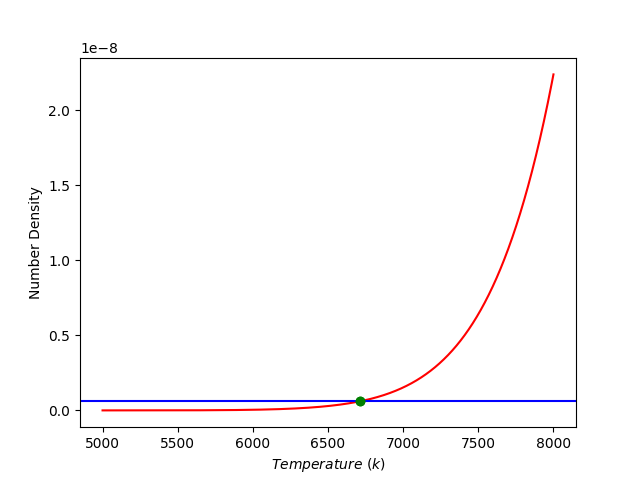
\includegraphics[width=14cm]{figure1.png}}}%
    \qquad
    \caption{Temperature vs. Number Density.}%
    \label{fig:example}%
\end{figure}


Figure 1 above shows Temperature vs. Number density. This problem defines the number density as $\eta = 6.1*10^{-10}$. The fraction of blackbody photons that have energy $hf < E_{0}$ as described in equation 2.44 is

$$
\frac{n(hf < E_{0})}{n_{\gamma}} \approx 0.42\Big(\frac{E_{0}}{kT}\Big)^{2}exp\Big(-\frac{E_{0}}{kT}\Big)
$$

or

$$
\eta \approx 0.42\Big(\frac{E_{0}}{kT}\Big)^{2}exp\Big(-\frac{E_{0}}{kT}\Big).
$$

Where $k$ is Boltzmann constant in $eV$, $E_{0}$ is $13.6 eV$, and $T$ is temperature. Plotting this function over an array of temperature values will result in a temperature value intersecting the line at $\eta = 6.1*10^{-10}$. Doing so give the results in Figure 1. The red line is the plot of the function defined above. The blue line is the horizontal line of the value $\eta$. The blue and red lines intersect at the green point. The green point is at the coordinates $T \approx 6714 k$ and $\eta = 6.1*10^{-10}$. Therefore, the temperature at which there will be one ionizing photon is

$$
\fbox{T = 6714 k}
$$

which is larger than the $T_{rec}$ temperature of $3760 k$.



\section*{Problem 8.4}
\begin{comment}
Assuming the benchmark model is correct, then the universe is know to be flat. Therefore, the luminosity distance for a flat universe is 

$$
d_{L} = S_{k}(r)(1 + z) = r(1 + z) = d_{p}(t_{0})(1 + z).
$$

Solving first for the proper distance, the book defines proper distance as

$$
d_{p}(t_{0}) = \frac{c}{H_{0}}z\Big[1 - \frac{1 + q_{0}}{2}z\Big]
$$

where $q_{0} \approx -0.53$ for the benchmark model given from the book. Furthermore, this number can be solved for using equation 6.11 where $q_{0} = \Omega_{r,0} + 1/2\Omega_{m,0} - \Omega_{\Lambda,0}$. For the benchmark universe $\Omega_{r,0} \approx 0, \Omega_{m,0} \approx 0.3, \Omega_{\Lambda,0} \approx 0.7$. This results in $q_{0} \approx -0.55$ which is close to the value the book gave just by approximating the benchmark values. The other values in this equation are the $z$ value where $z = 1090$, Hubble's constant $H_{0} = 70 km s^{-1}Mpc^{-1}$, and $c = 3.0*10^{8} m/s$. Converting $H_{0}$ form km to m gives us $H_{0} = 70000 m s^{-1}Mpc^{-1}$
\end{comment}



The last scattering surface is at redshift $z_{ls} = 1090$ much greater than 1. The approximation for $d_{A}$ is given by equation 6.40 as 

$$
d_{A} \approx \frac{d_{hor}(t_{0})}{z_{ls}}.
$$

This problem is based on the benchmark model. The current horizon distance is $d_{hor}(t_{0}) \approx 14000 Mpc$.

$$
d_{hor}(t_{0}) \approx 14000 Mpc.
$$

Therefore, we can find the angular-diameter distance using the equation above by 

$$
d_{A} \approx \frac{14000Mpc}{1090} \approx 12.8 Mpc.
$$

To find the luminosity distance the equation in terms of $d_{A}$ is given as

$$
d_{L} = d_{A}(1 + z)^{2} = 12.8 Mpc (1 + 1090)^{2} = 1.5*10^{7}Mpc.
$$

The proper distance for the Benchmark universe is gave in equation 6.37 as

$$
d_{p}(t_{0}) = d_{A}(1 + z) = \frac{d_{L}}{1 + z} = 12.8Mpc(1 + 1090) = 14000Mpc.
$$


\section*{Appendix}

\begin{lstlisting}[language=Python, caption= Problem 8.2 plotting code]
import numpy as np
import matplotlib.pyplot as plt

#----------------------------------# (Units)
E_0 = 13.6                         # eV
k = 8.617*10 ** -5                 # m^2kg/(s^2*k)
T = np.linspace(5000, 8000, 10000) # k
n = 6.1*10 ** (-10)                # Number Density (unitless)
#----------------------------------#

n_f = np.array(0.42 * (E_0/(k * T))*np.exp(-E_0/(k * T)))


plt.plot(T, n_f, 'r')
plt.axhline(y=n, color='b', linestyle='-')
for i in range(0, len(T)):
    if (n == round(n_f[i], 12)):
        plt.plot(T[i], n, 'go')
        print('The temperature is {}'
            .format(T[i]))
plt.xlabel(r'$Temperature \ (k)$')
plt.ylabel('Number Density')
plt.savefig('./figure1.png')
plt.show()
\end{lstlisting}


% --------------------------------------------------------------
%                           End Document.
% --------------------------------------------------------------
 
\end{document}

